\documentclass[12pt,a4paper]{article}\usepackage[]{graphicx}\usepackage[]{xcolor}
% maxwidth is the original width if it is less than linewidth
% otherwise use linewidth (to make sure the graphics do not exceed the margin)
\makeatletter
\def\maxwidth{ %
  \ifdim\Gin@nat@width>\linewidth
    \linewidth
  \else
    \Gin@nat@width
  \fi
}
\makeatother

\definecolor{fgcolor}{rgb}{0.345, 0.345, 0.345}
\newcommand{\hlnum}[1]{\textcolor[rgb]{0.686,0.059,0.569}{#1}}%
\newcommand{\hlsng}[1]{\textcolor[rgb]{0.192,0.494,0.8}{#1}}%
\newcommand{\hlcom}[1]{\textcolor[rgb]{0.678,0.584,0.686}{\textit{#1}}}%
\newcommand{\hlopt}[1]{\textcolor[rgb]{0,0,0}{#1}}%
\newcommand{\hldef}[1]{\textcolor[rgb]{0.345,0.345,0.345}{#1}}%
\newcommand{\hlkwa}[1]{\textcolor[rgb]{0.161,0.373,0.58}{\textbf{#1}}}%
\newcommand{\hlkwb}[1]{\textcolor[rgb]{0.69,0.353,0.396}{#1}}%
\newcommand{\hlkwc}[1]{\textcolor[rgb]{0.333,0.667,0.333}{#1}}%
\newcommand{\hlkwd}[1]{\textcolor[rgb]{0.737,0.353,0.396}{\textbf{#1}}}%
\let\hlipl\hlkwb

\usepackage{framed}
\makeatletter
\newenvironment{kframe}{%
 \def\at@end@of@kframe{}%
 \ifinner\ifhmode%
  \def\at@end@of@kframe{\end{minipage}}%
  \begin{minipage}{\columnwidth}%
 \fi\fi%
 \def\FrameCommand##1{\hskip\@totalleftmargin \hskip-\fboxsep
 \colorbox{shadecolor}{##1}\hskip-\fboxsep
     % There is no \\@totalrightmargin, so:
     \hskip-\linewidth \hskip-\@totalleftmargin \hskip\columnwidth}%
 \MakeFramed {\advance\hsize-\width
   \@totalleftmargin\z@ \linewidth\hsize
   \@setminipage}}%
 {\par\unskip\endMakeFramed%
 \at@end@of@kframe}
\makeatother

\definecolor{shadecolor}{rgb}{.97, .97, .97}
\definecolor{messagecolor}{rgb}{0, 0, 0}
\definecolor{warningcolor}{rgb}{1, 0, 1}
\definecolor{errorcolor}{rgb}{1, 0, 0}
\newenvironment{knitrout}{}{} % an empty environment to be redefined in TeX

\usepackage{alltt}
\usepackage{mypreamble}
\usepackage{myRpreamble}
\IfFileExists{upquote.sty}{\usepackage{upquote}}{}
\begin{document}
{\bf Arkaraj Mukherjee} \\
{\bf Homework 6}
\\
\begin{knitrout}
\definecolor{shadecolor}{rgb}{0.969, 0.969, 0.969}\color{fgcolor}\begin{kframe}
\begin{alltt}
\hlkwd{library}\hldef{(}\hlsng{"tidyverse"}\hldef{);}
\end{alltt}
\end{kframe}
\end{knitrout}
\begin{enumerate}[label=\arabic*.]
	\item
	\begin{enumerate}[label=(\alph*)]
	\item The probability mass function of this empirical distribution is
		$$p(x) = \begin{cases}\frac{1}{10}\text{ if }x\in\{13,40,23,15,21,4,44,16,32,14\}\end{cases}$$
	and the ECDF is
	$$F(x) =
	\begin{cases}
	0\text{ if }x<4\\
	\frac{1}{10}\text{ if }4\leq x<13\\
	\frac{2}{10}\text{ if }13\leq x<14\\
	\frac{3}{10}\text{ if }14\leq x<15\\
	\frac{4}{10}\text{ if }14\leq x<16\\
	\frac{5}{10}\text{ if }16\leq x<21\\
	\frac{6}{10}\text{ if }21\leq x<23\\
	\frac{7}{10}\text{ if }23\leq x<32\\
	\frac{8}{10}\text{ if }32\leq x<40\\
	\frac{9}{10}\text{ if }40\leq x<44\\
	1\text{ if }x\geq 44
	\end{cases}$$
	\item
\begin{knitrout}
\definecolor{shadecolor}{rgb}{0.969, 0.969, 0.969}\color{fgcolor}\begin{kframe}
\begin{alltt}
\hldef{dat} \hlkwb{=} \hlkwd{c}\hldef{(}\hlnum{13}\hldef{,}\hlnum{40}\hldef{,}\hlnum{23}\hldef{,}\hlnum{15}\hldef{,}\hlnum{21}\hldef{,}\hlnum{4}\hldef{,}\hlnum{44}\hldef{,}\hlnum{16}\hldef{,}\hlnum{32}\hldef{,}\hlnum{14}\hldef{)}
\hldef{F} \hlkwb{=} \hlkwd{ecdf}\hldef{(dat)}
\hldef{x}\hlkwb{=}\hlopt{-}\hlnum{5}\hlopt{:}\hlnum{60}\hldef{;}
\hldef{ECDF}\hlkwb{=}\hlkwd{F}\hldef{(x);}
\hldef{EPDF}\hlkwb{=}\hlkwd{F}\hldef{(x)}\hlopt{-}\hlkwd{F}\hldef{(x}\hlopt{-}\hlnum{1}\hldef{);}
\hlkwd{plot}\hldef{(x,ECDF,}\hlkwc{type}\hldef{=}\hlsng{"s"}\hldef{,}\hlkwc{col}\hldef{=}\hlsng{"blue"}\hldef{,}\hlkwc{ylim}\hldef{=}\hlkwd{c}\hldef{(}\hlopt{-}\hlnum{0.01}\hldef{,}\hlnum{1.01}\hldef{),}\hlkwc{lwd}\hldef{=}\hlnum{2}\hldef{)}
\hlkwd{lines}\hldef{(x,EPDF,}\hlkwc{type}\hldef{=}\hlsng{"p"}\hldef{,}\hlkwc{pch}\hldef{=}\hlnum{16}\hldef{,}\hlkwc{col}\hldef{=}\hlsng{"red"}\hldef{)}
\hlkwd{legend}\hldef{(}\hlsng{"topleft"}\hldef{,}\hlkwc{legend}\hldef{=}\hlkwd{c}\hldef{(}\hlsng{"ECDF"}\hldef{,}\hlsng{"EPDF"}\hldef{),}\hlkwc{col}\hldef{=}\hlkwd{c}\hldef{(}\hlsng{"blue"}\hldef{,}\hlsng{"red"}\hldef{),}
\hlkwc{pch}\hldef{=}\hlkwd{c}\hldef{(}\hlnum{NA}\hldef{,}\hlnum{16}\hldef{),}\hlkwc{lty}\hldef{=}\hlkwd{c}\hldef{(}\hlnum{1}\hldef{,}\hlnum{NA}\hldef{))}
\end{alltt}
\end{kframe}
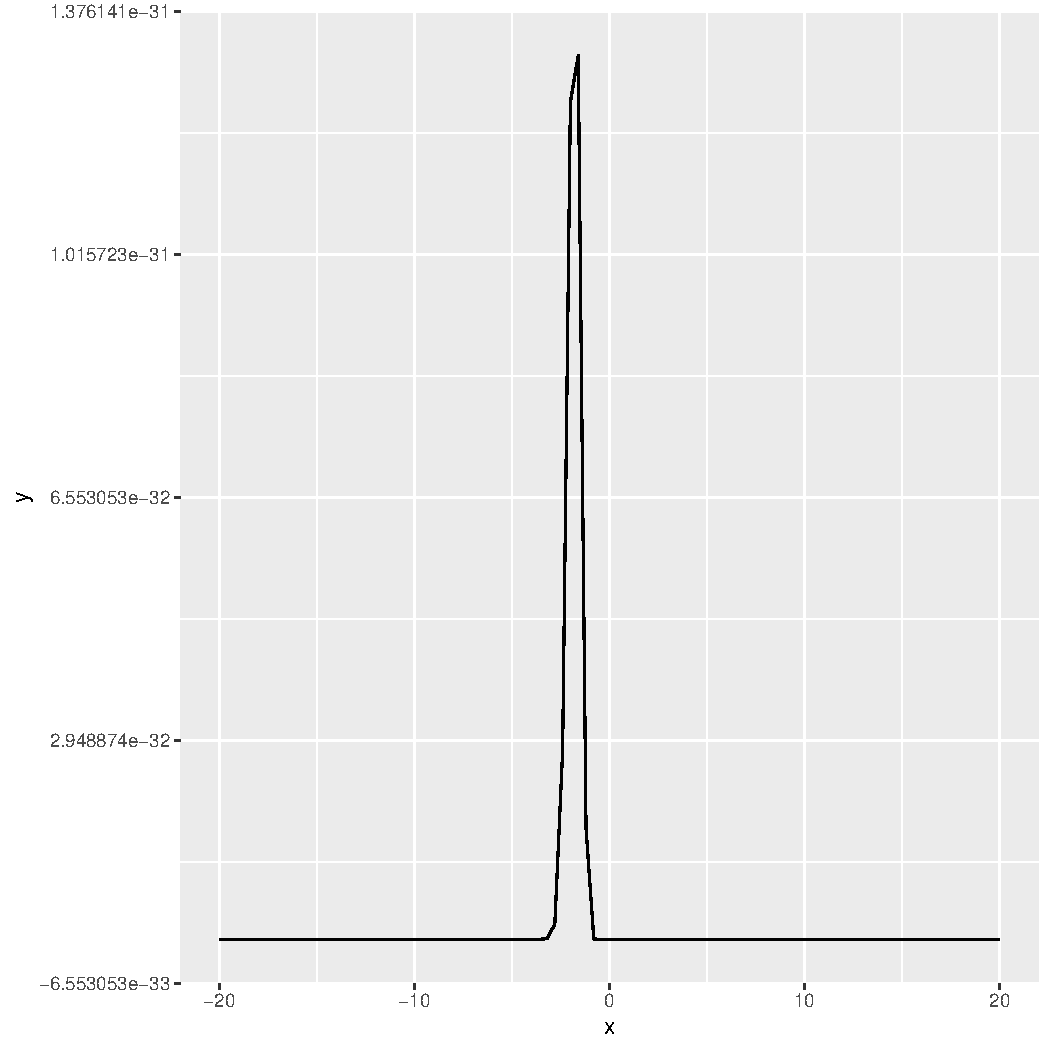
\includegraphics[width=\maxwidth]{figure/unnamed-chunk-2-1} 
\end{knitrout}
	\end{enumerate}
	\item NA

	\item 
	Its known that if $X\sim\text{Unif}(a,b)$ then $\mathbf{E}[X]=(a+b)/2$
	and $\mathbf{E}[X^2]=(a^2+ab+b^2)/3$. Using method of moments, we find
	$\hat{a},\hat{b}$ as usual,
	$$\frac{1}{n}\sum_{i=1}^nX_i=\frac{\hat{a}+\hat{b}}{2}\text{ and
	}\frac{1}{n}\sum_{i=1}^nX_i^2=\frac{\hat{a}^2+\hat{a}\hat{b}+\hat{b}^2}{3}$$
	We write $a,b$ and omit the hats for ease of typesetting. Here,
	$a^2+ab+b^2=(a+b)^2-ab$ and $a+b=2\mathbf{E}[X]$, which gives us
	$ab=(2\mathbf{E}[X])^2-3\mathbf{E}[X^2]$ which implies that $a,b$ are
	roots of the quadratic
	$f(y)=y^2-2\mathbf{E}[X]y+(4\mathbf{E}[X]^2-3\mathbf{E}[X^2])$. Thus,
	them being equal is equivalent to this quadratic having discriminant
	$0$, i.e.
	$4\mathbf{E}[X]^2-4\cdot(4\mathbf{E}[X]^2-3\mathbf{E}[X^2])=0$,
	rearranging which we arrive at $\mathbf{E}[X^2]=\mathbf{E}[X]^2$ which
	is again equivalent to the sampl variance being $0$ which happens if
	and only if all the data points in the empirical realisation having the
	exact same value so we are done.
	\item 
	\begin{enumerate}[label=(\alph*)]
        \item 
\begin{knitrout}
\definecolor{shadecolor}{rgb}{0.969, 0.969, 0.969}\color{fgcolor}\begin{kframe}
\begin{alltt}
\hldef{n} \hlkwb{=} \hlnum{100}
\hldef{N} \hlkwb{=} \hlnum{20}
\hldef{p} \hlkwb{=} \hlnum{0.4}
\hldef{x} \hlkwb{=} \hlkwd{rbinom}\hldef{(n,N,p)}
\hldef{m1} \hlkwb{=} \hlkwd{mean}\hldef{(x)}
\hldef{m2} \hlkwb{=} \hlkwd{mean}\hldef{(x}\hlopt{^}\hlnum{2}\hldef{)}
\hldef{Nhat} \hlkwb{=} \hldef{m1}\hlopt{^}\hlnum{2} \hlopt{/} \hldef{(m1} \hlopt{-} \hldef{(m2} \hlopt{-} \hldef{m1}\hlopt{^}\hlnum{2}\hldef{))}
\hldef{phat} \hlkwb{=} \hldef{(m1} \hlopt{-} \hldef{(m2} \hlopt{-} \hldef{m1}\hlopt{^}\hlnum{2}\hldef{))} \hlopt{/} \hldef{m1}
\hldef{Nhat} \hlopt{-} \hldef{N}
\end{alltt}
\begin{verbatim}
## [1] 4.438028
\end{verbatim}
\begin{alltt}
\hldef{phat} \hlopt{-} \hldef{p}
\end{alltt}
\begin{verbatim}
## [1] -0.06977695
\end{verbatim}
\end{kframe}
\end{knitrout}
        \item 
\begin{knitrout}
\definecolor{shadecolor}{rgb}{0.969, 0.969, 0.969}\color{fgcolor}\begin{kframe}
\begin{alltt}
\hldef{n} \hlkwb{=} \hlnum{1000}
\hldef{N} \hlkwb{=} \hlnum{20}
\hldef{p} \hlkwb{=} \hlnum{0.4}
\hldef{x} \hlkwb{=} \hlkwd{rbinom}\hldef{(n,N,p)}
\hldef{m1} \hlkwb{=} \hlkwd{mean}\hldef{(x)}
\hldef{m2} \hlkwb{=} \hlkwd{mean}\hldef{(x}\hlopt{^}\hlnum{2}\hldef{)}
\hldef{Nhat} \hlkwb{=} \hldef{m1}\hlopt{^}\hlnum{2} \hlopt{/} \hldef{(m1} \hlopt{-} \hldef{(m2} \hlopt{-} \hldef{m1}\hlopt{^}\hlnum{2}\hldef{))}
\hldef{phat} \hlkwb{=} \hldef{(m1} \hlopt{-} \hldef{(m2} \hlopt{-} \hldef{m1}\hlopt{^}\hlnum{2}\hldef{))} \hlopt{/} \hldef{m1}
\hldef{Nhat} \hlopt{-} \hldef{N}
\end{alltt}
\begin{verbatim}
## [1] -1.488499
\end{verbatim}
\begin{alltt}
\hldef{phat} \hlopt{-} \hldef{p}
\end{alltt}
\begin{verbatim}
## [1] 0.03389243
\end{verbatim}
\end{kframe}
\end{knitrout}
        It does change, the error is much smaller now.
        \item 
\begin{knitrout}
\definecolor{shadecolor}{rgb}{0.969, 0.969, 0.969}\color{fgcolor}\begin{kframe}
\begin{alltt}
\hldef{n} \hlkwb{=} \hlnum{100}\hldef{;}
\hldef{N} \hlkwb{=} \hlnum{10}\hldef{;}
\hldef{p} \hlkwb{=} \hlnum{0.9}\hldef{;}
\hldef{x} \hlkwb{=} \hlkwd{rbinom}\hldef{(n,N,p);}
\hldef{m1} \hlkwb{=} \hlkwd{mean}\hldef{(x);}
\hldef{m2} \hlkwb{=} \hlkwd{mean}\hldef{(x}\hlopt{^}\hlnum{2}\hldef{);}
\hldef{Nhat} \hlkwb{=} \hldef{m1}\hlopt{^}\hlnum{2} \hlopt{/} \hldef{(m1} \hlopt{-} \hldef{(m2} \hlopt{-} \hldef{m1}\hlopt{^}\hlnum{2}\hldef{));}
\hldef{phat} \hlkwb{=} \hldef{(m1} \hlopt{-} \hldef{(m2} \hlopt{-} \hldef{m1}\hlopt{^}\hlnum{2}\hldef{))} \hlopt{/} \hldef{m1;}
\hldef{Nhat} \hlopt{-} \hldef{N}
\end{alltt}
\begin{verbatim}
## [1] 0.1954023
\end{verbatim}
\begin{alltt}
\hldef{phat} \hlopt{-} \hldef{p}
\end{alltt}
\begin{verbatim}
## [1] -0.03
\end{verbatim}
\begin{alltt}
\hldef{n} \hlkwb{=} \hlnum{1000}\hldef{;}
\hldef{N} \hlkwb{=} \hlnum{10}\hldef{;}
\hldef{p} \hlkwb{=} \hlnum{0.9}\hldef{;}
\hldef{x} \hlkwb{=} \hlkwd{rbinom}\hldef{(n,N,p);}
\hldef{m1} \hlkwb{=} \hlkwd{mean}\hldef{(x);}
\hldef{m2} \hlkwb{=} \hlkwd{mean}\hldef{(x}\hlopt{^}\hlnum{2}\hldef{);}
\hldef{Nhat} \hlkwb{=} \hldef{m1}\hlopt{^}\hlnum{2} \hlopt{/} \hldef{(m1} \hlopt{-} \hldef{(m2} \hlopt{-} \hldef{m1}\hlopt{^}\hlnum{2}\hldef{));}
\hldef{phat} \hlkwb{=} \hldef{(m1} \hlopt{-} \hldef{(m2} \hlopt{-} \hldef{m1}\hlopt{^}\hlnum{2}\hldef{))} \hlopt{/} \hldef{m1;}
\hldef{Nhat} \hlopt{-} \hldef{N}
\end{alltt}
\begin{verbatim}
## [1] 0.006464389
\end{verbatim}
\begin{alltt}
\hldef{phat} \hlopt{-} \hldef{p}
\end{alltt}
\begin{verbatim}
## [1] 0.000717741
\end{verbatim}
\end{kframe}
\end{knitrout}
	\end{enumerate}
	\item
	\begin{enumerate}[label=(\alph*)]
	\item There is a possibility that the sample mean is $1$, which causes
		divison by zero below if left unattended. This occurs if and
		only if all the samples are $1$, in which case $\mL(=p,\text{
		which follows from the expression deduced below})$ is not
		maximised by any $p\in (0,1)$ so we assume henceforth that the
		sample mean is not $1$. The likelihood function is,
	$$\mL(p;X_1,\ldots,X_n)=\prod_{i=1}^np(1-p)^{X_i-1}=p^n(1-p)^{n\overline{X}-n}$$
	where $\overline{X}$ is the sample mean. 
	\item $$l(p;X_1,\ldots,X_n)=n\log(p)+(n\overline{X}-n)\log(1-p)$$
	This is a continuous function in $p$, on $(0,1)$ and we will find the
	point where it attains the maximum value using the double derivative
	test.
	$$\frac{d
	l}{dp}=\frac{n}{p}-\frac{n\overline{X}-n}{1-p}=0\implies\frac{1}{p}=\frac{\overline{X}-1}{1-p}\implies\overline{X}-1=\frac{1}{p}-1\implies
	p=\frac{1}{\overline{X}}$$
	$$\frac{d^2l}{dp^2}\bigg|_{p=1/\overline{X}}=-\frac{n}{p^2}-\frac{n\overline{X}-n}{(1-p)^2}\bigg|_{p=1/\overline{X}}=-n\overline{X}^2-\frac{n\overline{X}^2}{\overline{X}-1}<0$$thus, we have shown that $l$ is maximised at $p=1/\overline{X}$.
\item As $\log$ is a strictly increasing function on its domain, we see that,
	$$\argmax_{p\in(0,1)}\mL(p;X_1,\ldots,X_n)=\argmax_{p\in(0,1)}\log\mL(p;X_1,\ldots,X_n)=\frac{1}{\overline{X}}$$
	and thus, the maximum likelihood estimate for $p$ is $1/\overline{X}$
	
	\end{enumerate}
\end{enumerate}
\end{document}
